\section{Обзор предметной области}
В данном разделе будет произведён обзор предметной области задачи, решаемой в рамках дипломного проекта; рассмотрены вопросы о сущности
байесовых сетей и принципе их работы; приведена оценка сложности различных проблем, возникающих при применении вероятностных сетей для
решения прикладных задач. Также будут рассмотрены принципы работыалгоритмов вывода структуры по данным, реализованных
в программномобеспечении разработанном в рамках дипломного проекта, и произведеносравнение с существующим ПО для решения схожих задач.

\subsection{API как средство интеграции приложений}
API определяет функциональность, которую предоставляет программа (модуль, библиотека), при этом API позволяет абстрагироваться от того, как именно эта функциональность реализована.

Если программу (модуль, библиотеку) рассматривать как чёрный ящик, то API — это множество «ручек», которые доступны пользователю данного ящика, и которые он может вертеть и дёргать.

Программные компоненты взаимодействуют друг с другом посредством API. При этом обычно компоненты образуют иерархию — высокоуровневые компоненты используют API низкоуровневых компонентов, а те, в свою очередь, используют API ещё более низкоуровневых компонентов.

По такому принципу построены протоколы передачи данных по Интернет. Стандартный стек протоколов (сетевая модель OSI) содержит 7 уровней (от физического уровня передачи бит до уровня протоколов приложений, подобных протоколам HTTP и IMAP). Каждый уровень пользуется функциональностью предыдущего уровня передачи данных и, в свою очередь, предоставляет нужную функциональность следующему уровню.

Важно заметить, что понятие протокола близко по смыслу к понятию API. И то, и другое является абстракцией функциональности, только в первом случае речь идёт о передаче данных, а во втором — о взаимодействии приложений.
API библиотеки функций и классов включает в себя описание сигнатур и семантики функций.


\subsection{Проблемы, связанные с многообразием API}
Практически все операционные системы (UNIX, Windows, Mac OS и т. д.) имеют API, с помощью которого программисты могут создавать приложения для этой операционной системы. Главный API операционных систем — это множество системных вызовов.

В индустрии программного обеспечения общие стандартные API для стандартной функциональности имеют важную роль, так как они гарантируют, что все программы, использующие общий API, будут работать одинаково хорошо или, по крайней мере, типичным привычным образом. В случае API графических интерфейсов это означает, что программы будут иметь похожий пользовательский интерфейс, что облегчает процесс освоения новых программных продуктов.

С другой стороны, отличия в API различных операционных систем существенно затрудняют перенос приложений между платформами. Существуют различные методы обхода этой сложности — написание «промежуточных» API (API графических интерфейсов WxWidgets, Qt, GTK и т. п.), написание библиотек, которые отображают системные вызовы одной ОС в системные вызовы другой ОС (такие среды исполнения, как Wine, cygwin и т. п.), введение стандартов кодирования в языках программирования (например, стандартная библиотека языка C), написание интерпретируемых языков, реализуемых на разных платформах (sh, python, perl, php, tcl, Java и т. д.).

Также необходимо отметить, что в распоряжении программиста часто находится несколько различных API, позволяющих добиться одного и того же результата. При этом каждый API обычно реализован с использованием API программных компонент более низкого уровня абстракции.

Например: для того, чтобы увидеть в браузере строчку «Hello, world!», достаточно лишь создать HTML-документ с минимальным заголовком и простейшим телом, содержащим данную строку. Когда браузер откроет этот документ, программа-браузер передаст имя файла (или уже открытый дескриптор файла) библиотеке, обрабатывающей HTML-документы, та, в свою очередь, при помощи API операционной системы прочитает этот файл и разберётся в его устройстве, затем последовательно вызовет через API библиотеки стандартных графических примитивов операции типа «очистить окошко», «написать “Hello, world!” выбранным шрифтом». Во время выполнения этих операций библиотека графических примитивов обратится к библиотеке оконного интерфейса с соответствующими запросами, уже эта библиотека обратится к API операционной системы, чтобы записать данные в буфер видеокарты.

При этом практически на каждом из уровней реально существует несколько возможных альтернативных API. Например: мы могли бы писать исходный документ не на HTML, а на LaTeX, для отображения могли бы использовать любой браузер. Различные браузеры, вообще говоря, используют различные HTML-библиотеки, и, кроме того, всё это может быть (вообще говоря) собрано с использованием различных библиотек примитивов и на различных операционных системах.

Основными сложностями существующих многоуровневых систем API, таким образом, являются:
\begin{enumerate}
    \item сложность портирования программного кода с одной системы API на другую (например, при смене ОС);
    \item потеря функциональности при переходе с более низкого уровня на более высокий. Грубо говоря, каждый «слой» API создаётся для облегчения выполнения некоторого стандартного набора операций. Но при этом реально затрудняется, либо становится принципиально невозможным выполнение некоторых других операций, которые предоставляет более низкий уровень API.
\end{enumerate}



\subsection{Балансировка нагрузки}

Балансировка нагрузки  - миграции процессов или выбор компьютера для запуска нового процесса с целью равномерной загрузки всех компьютеров в вычислительной системе, оптимизации использования ресурсов и сокращения времени вычисления.

Балансировка нагрузки может быть использована для расширения возможностей компьютерной системы, состоящей более чем из одного сервера. Она также может позволить продолжать работу даже в условиях, когда несколько серверов вышли из строя. Благодаря этому растёт отказоустойчивость.

В системах с большим числом узлов часто возникают сбои, требующие вмешательства человека и временного отключения компьютера. Количество сбоев растёт пропорционально числу узлов. При этом необходимо, чтобы вычисления продолжались, так как зачастую расчётные программы не обладают встроенной возможностью сохранить своё состояние или из-за того, что результат нужно получить как можно быстрее. Здесь также возникает необходимость перенести работающий процесс на другой компьютер.

Аналогичная проблема возникает при совместном использовании группы компьютеров и в качестве кластера, и в качестве учебной аудитории. (Такое использование типично для учебных заведений.) Когда начинаются занятия, требуется освободить часть компьютеров для студентов и преподавателя, перенеся с них задачи на другие машины. При этом не всегда заранее известно, сколько машин понадобится.

Cистемы балансировки нагрузки применяются на серверных кластерах, межсетевых экранах, серверах инспектирования содержания (например, антивирусных и антиспамовых фильтрах) – всюду, где задача может быть разделена на параллельные слабо связанные задачи, требования которых к ресурсам могут переменными и даже труднопредсказуемыми. Под слабой связанностью подразумевается отсутствие необходимости частого обмена данными между процессами.

Система балансировки нагрузки должна постоянно отслеживать уровень нагрузки и состояние управляемых компьютеров с тем, чтобы на основании собранной информации в любой момент выбирать для  запуска или переноса очередного процесса  к тот сервер, на котором процесс сможет наилучшим образом работать.

\subsubsection{Балансировка нагрузки Web-серверов}

Cистема балансировки нагрузки Web-серверов - это инструментальное средство, выполненное в виде сетевого  устройства или программы и предназначенное для переадресации клиентских запросов на наименее загруженный или наиболее подходящий Web-сервер из группы машин, на которых хранятся зеркальные копии информационного ресурса [8]. Вся система представляются клиенту в виде некоего единого виртуального сервера. Возможность переноса запроса с одного сервера на другой не предусматривается.

\begin{figure}
  \centering
  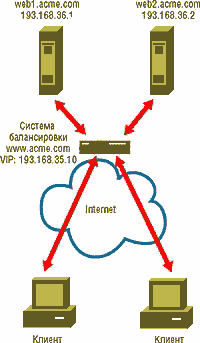
\includegraphics[width=0.3\textwidth]{images/balance-sys.png}
  \caption{Система балансировки нагрузки на 2 web-сервера}
\end{figure}

Для работы такой системы необходим алгоритм выбора сервера. Обычно в таких системах выбор происходит по принципу кругового списка, что эффективно в случае и одинаковых серверов и запросов, требующих одинаковое количество ресурсов.

\subsubsection{Избыточные системы балансировки}

Системы балансировки нагрузки - средства доступа к серверам Web, и потому выход такого средства из строя может повлечь за собой полное прекращение работы узла. Отсюда вывод: при планировании и реализации инфраструктуры с выравниванием нагрузок важно принимать во внимание отказоустойчивость средств балансировки, а также выбирать решения с широкой полосой пропускания, способные обеспечить высокую производительность системы в целом. В распоряжении администратора имеются две схемы организации избыточных систем балансировки нагрузки: первая предполагает, что одна система балансировки функционирует в активном режиме, а другая - находится в состоянии ожидания (active-and-standby type); вторая же схема предусматривает одновременное функционирование обеих систем балансировки (active-and-active type). Обе схемы предполагают наличие на одном узле двух экземпляров систем балансировки нагрузки.

При использовании метода одна система активна, а другая находится в состоянии ожидания, резервная система балансировки постоянно контролирует состояние главной системы, и, как только она  выходит из строя,  резервная система балансировки принимает на себя функции главной. Когда же главная система возобновляет работу, резервная передает ей управление трафиком и вновь переходит в режим ожидания.

В схеме с двумя активными системами балансировки нагрузки обе системы обслуживают трафик и подстраховывают друг друга. Представим для примера узел Web, состоящий из четырех серверов. Два из них обслуживаются первой системой балансировки нагрузки, и два - второй. Когда одна система балансировки выходит из строя, заботу обо всех четырех серверах берет на себя вторая система. Этот метод в полной мере использует ресурсы средств балансировки и повышает производительность узла.

\subsubsection{Больше, чем технология}

Компании, которые обслуживают информационные центры Web и занимаются электронной коммерцией, - далеко не единственные организации, применяющие системы балансировки нагрузки для управления трафиком и поддержания порядка в своих виртуальных хозяйствах. Многие компании взяли на вооружение средства балансировки для того, чтобы повысить производительность и доступность своих узлов Web.

Системы выравнивания нагрузки обеспечивают мониторинг нагрузок и состояния серверов, правильный выбор из пула серверов машины, способной наилучшим образом обработать запрос клиента, а также управление трафиком как внутри узла, так и в глобальном масштабе. Благодаря этому они становятся мощным оружием в конкурентной борьбе между компаниями, открывшими свои представительства в киберпространстве.

\subsection{Мониторинг состояния серверов}

\subsubsection{Внешний мониторинг}

При проведении внешнего мониторинга система балансировки нагрузки рассчитывает время отклика сервера, для чего направляет на сервер запрос и замеряет время ответа, например, по протоколу управления сообщениями Internet Control Message Protocol (ICMP).  Эти тесты позволяют системе проверить  готовность сервера к работе и узнать, сколько времени необходимо для передачи информации с сервера на систему балансировки и обратно. Если система балансировки нагрузки не получает отклика от сервера после нескольких последовательных запросов, считается, что данный сервер недоступен, работает с большой нагрузкой или произошёл какой-либо сбой.

Чтобы убедиться в правильности функционирования стека TCP сервера, система балансировки нагрузки предпринимает попытку установить соединение по протоколу TCP, для чего требуется осуществить состоящий из трех этапов обмен подтверждающими сообщениями. Сначала серверу направляется TCP-пакет, в котором значение бита SYN установлено равным 1. Если после этого система балансировки получает от сервера TCP-пакет, в котором значение бита SYN равно 1, а значение бита ACK тоже установлено равным 1, она направляет серверу второй TCP-пакет со значением бита SYN равным 0 и значением бита ACK равным 1. Если обмен подтверждающими сообщениями завершился успешно, значит, TCP-стек сервера функционирует нормально. Качество TCP-соединения с сервером оценивается системой как время, необходимое для выполнения всех трех этапов обмена подтверждающими сообщениями.

Лучшие средства балансировки нагрузки могут обеспечивать мониторинг времени отклика и готовности как самого Web-сервера, так и установленных на нем приложений еще одним способом: на сервер направляется запрос по протоколу HTTP на получение информационных материалов или адреса URL. Пусть именем начальной страницы сервера web1.kto-to.com будет index.html. Система балансировки нагрузки на рисунке 1.1 может инициировать предусмотренную по протоколу HTTP команду Get, запрашивая тем самым у сервера web1.kto-to.com содержимое страницы index.html. Если код возврата, направляемый системе Web-сервером, будет 200, значит, начальная страница на сервере web1.kto-to.com недоступна. Время отклика определяется системой балансировки нагрузки как время с момента отправки запроса на предоставление информации до момента получения кода возврата.

\subsubsection{Внутренний мониторинг}

Подробную информацию о таких существенных характеристиках сервера, как состояние центрального процессора, памяти, системной шины, шины ввода/вывода, сетевой интерфейсной платы, а также о ряде важных ресурсов системы и прикладных программ  может предоставить только внутренний мониторинг. Агенты, которые устанавливаются на каждом сервере, постоянно контролируют состояние своего компьютера и сообщают о нем системе балансировки. Внутренний мониторинг широко применяется в программных системах балансировки, но в аппаратных устройствах и в решениях на базе коммутаторов этот метод диагностики реализуется редко.

\subsection{Задача определения неисправности или отказа того или иного модуля системы}

В сложных распределённых системах одновременно выполняется множество операций, и в случае возникновения неисправности или отказа того или иного модуля системы бывает достаточно сложно сразу же определить причину неисправности или отказа. Поэтому важно наличие централизованного механизма получения и хранения сообщений и протоколов о работе программных модулей и подсистем в составе любого программного комплекса.

Каждый модуль системы, выполнив ту или иную операцию, должен добавить запись в соответствующий журнал операций. Использование журналов операций сокращает время на поиск причин возникающих неисправностей, так как становится возможным однозначно определить, после выполнения какой операции произошёл отказ.

Поскольку комплексы программ независимо от своей прикладной сферы должны иметь средства протоколирования операций, то целесообразно создать универсальный компонент для ведения журнала операций с возможностью подключать его к различным программам.

\newpage
